\documentclass[a4paper,11pt,titlepage,abstract,numbers=noenddot,automark,mnsy,intlimits,rgb,dvipsnames]{report}
\usepackage[hidelinks, colorlinks=true, urlcolor=blue, linkcolor=black, citecolor=blue]{hyperref}
\usepackage[english]{babel}
\usepackage{unicode-math}
\usepackage{xunicode}
\usepackage{url}
\usepackage{cite}
\usepackage{graphicx}
\usepackage[justification=centering, labelfont=bf]{caption}
\usepackage{float}
\usepackage{pgfgantt}
\usepackage{marvosym}
\usepackage{siunitx}
\usepackage{multirow}
\usepackage[nottoc]{tocbibind}
\usepackage{indentfirst}
\usepackage{afterpage}
\usepackage{minted}
\usepackage{tabularx}
\usepackage{tikz}
\usepackage[toc,page]{appendix}
\usetikzlibrary{arrows,positioning}
\usepackage{fontspec}
\usepackage{parskip}
\usepackage{fancyhdr}
\usepackage{titlesec}

\defaultfontfeatures{Scale=MatchLowercase}
\setmainfont[Ligatures=TeX,
BoldFont=texgyrepagella-bold.otf,
BoldItalicFont=texgyrepagella-bolditalic.otf,
ItalicFont=texgyrepagella-italic.otf]{texgyrepagella-regular.otf}
\setsansfont[Ligatures=TeX,
BoldFont=lmsans10-bold.otf,
BoldItalicFont=lmsans10-boldoblique.otf,
ItalicFont=lmsans10-oblique.otf]{lmsans10-regular.otf}
\setmonofont[BoldFont=lmmonolt10-bold.otf,
BoldItalicFont=lmmonolt10-boldoblique.otf,
ItalicFont=lmmono10-italic.otf,
SlantedFont=lmmonoslant10-regular.otf]{lmmono10-regular.otf}
\setmathfont{texgyrepagella-math.otf}
\setmathfont[range={\mathcal,\mathbfcal},StylisticSet=1]{xits-math.otf}
\setlength{\parindent}{24pt}
\setcounter{secnumdepth}{5}
\setcounter{tocdepth}{1}


 
\pagestyle{fancy}
\fancyhf{}
\fancyhead[LE,RO]{Héctor Ramón}
\fancyhead[RE,LO]{\leftmark}
\fancyfoot[RE]{Final degree project}
\fancyfoot[LO]{\emph{Web platform for multiplayer programming games}}
\fancyfoot[LE,RO]{\thepage}

\renewcommand{\footrulewidth}{0.5pt}
\setlength{\marginparwidth}{0pt}
\setlength{\parskip}{0.8em}


\titleformat{\chapter}{\normalfont\bfseries}{\Huge\thechapter}{20pt}{\Huge}
\newcommand*{\fullref}[1]{\hyperref[{#1}]{\autoref*{#1} \nameref*{#1}}}

\begin{document}
\begin{titlepage}
\begin{center}
\textsc{\Large Degree Final Project}
\\[1.5cm]
\rule{\linewidth}{0.5mm}
\\[0.4cm]
{\huge
\bfseries
Web platform for massive multiplayer programming games
\\[0.4cm]
}
\rule{\linewidth}{0.5mm}
\\[2.5cm]
\begin{center}
\large
Héctor Ramón Jiménez
\end{center}
Directed by Jordi Petit Silvestre
\vfill
{\large
Facultat d'Informàtica de Barcelona
}
\\[0.5cm]
{\large
\today
}
\end{center}
\end{titlepage}
\clearpage
\begin{abstract}
...
\end{abstract}
\clearpage
\tableofcontents
\clearpage
\chapter{Introduction}
\section{Brief history}
\subsection{Playing games while programming}
In 1961, \textbf{Victor Vyssotsky}, a mathematician and computer scientist working at Bell Labs, had an idea. He devised
a computer game, but not a traditional one where the player inputs the different actions from a controller to play it.
No. He wanted to create a game that it could only be played by writing a \textbf{computer program}. And so, along with \textbf{Robert
Morris Sr.} and \textbf{Doug McIlroy}, they created \textbf{Darwin} \cite{darwin}: the first programming game.

A \textbf{programming game} is a computer game where the player does not directly interact with the game. Instead, the
player writes a \textbf{computer program} that plays the game. These \textbf{computer programs} are usually called \textbf{artifficial
intelligences} (\textbf{\texttt{AI}}s) because they try to make intelligent decisions to win the game.

\textbf{Darwin} consisted of two or more small programs, written by the players, that were loaded in memory. The main goal
of the game was to spread copies of your own program and find and kill the copies of other players. The game was only
played for a few weeks before Morris developed an ultimate program, as no-one managed to produce anything that could
defeat it.

Since then, many other programming games have been created \cite{pg}. Some of them are even commercial games, like
\textbf{SpaceChem} \cite{spacechem}.
\subsection{Playing with other people}
With the arrival of the \textbf{Internet} and the \textbf{W}orld \textbf{W}ide \textbf{W}eb, there was nothing stopping people from
developing web platforms for \textbf{multiplayer programming games}.

A \textbf{multiplayer programming game} is a \textbf{programming game} where multiple players compete with each other to win the
game. Thus, the game becomes a challenge where strategy and programming skills make the difference.

These web platforms allow players to compete with each other easily. For example, \textbf{Robot Game}
\cite{robotgame} is a website where anyone can upload an \textbf{\texttt{AI}} written in \texttt{Python} and compete with other people.
\subsection{Playing while learning}
Writing \textbf{\texttt{AI}}s can be a really fun and rewarding experience because the game allows the players to see how their
\textbf{algorithms work visually}, while competition motivates them to \textbf{learn and improve}.

It is not a surprise, then, that programming games are being used in schools to teach students different programming
techniques. For instance, an \textbf{\texttt{AI} programming challenge} is held every semester in the \textbf{Barcelona School of
Informatics} (\textbf{FIB}) where students enrolled in the subject \textbf{Data Structures and Algorithms} (\textbf{EDA}) \cite{eda}
compete with each other in a multiplayer programming game using the \textbf{Jutge} platform \cite{jutge}.
\section{Personal motivation}
\textbf{I love videogames}. Ever since my father introduced me to my first computer when I was 3 years old.
I was immediately hooked. I started playing simple puzzle games, while discovering first person shooters and strategic
games soon after.

\textbf{Videogames were the main reason I chose to study computer science}. I learned my first
programming language (\textbf{\texttt{PHP}}) because I wanted to open a website
to share my passion about videogames. I was 10 years old back then. \textbf{Programming} has been a really important
aspect of my life.

\textbf{Studying computer science has made me love videogames even more}. When I a see videogame now, I can try to
imagine the logic
behind it. I can try to picture the different algorithms involved. I imagine thousands of bits correctly aligned,
flowing and changing constantly, while they follow some complex logic. For me, the fact that a \textbf{videogame} is
able to show how its code works \textbf{visually} is truly fascinating.

Programming games mix together two of my passions: \textbf{videogames} and \textbf{programming}. [...]
\section{Summary}
This report consists of three different parts. Each one of them describes a vital phase in the development of
the project:
\begin{description}
\item[Formulation]
It identifies and analyzes the \textbf{problem to solve}, it \textbf{specifies} the scope of
  the project, and it shows the \textbf{design} of the solution.
\item[Implementation]
It describes the development of the different \textbf{components} that compose the solution.
\item[Review]
It describes the \textbf{validation methodology}, it states the final \textbf{planning} and \textbf{economic cost}
  of the project, and it discusses the \textbf{sustainability} and \textbf{legality} of the project.
\end{description}
\part{Formulation}
\chapter{Analysis}
\section{State of the art}
Current multiplayer programming games feature \textbf{short matches} with a \textbf{small number of players}. There
is no way to perform a challenge with a considerable amount of students playing at the same time. Therefore, multiple
matches are necessary to decide who wrote the best program.
\section{The future}
Multiplayer programming games need to evolve. They need to feature \textbf{huge worlds}, \textbf{long matches} and
a \textbf{massive amount of players in real-time}. Then, players will feel attached to the match, programs will need to
\textbf{adapt} constantly as they play with \textbf{everyone at the same time}. It is time to take this genre to the next level and
create \textbf{massive multiplayer programming games} (\textbf{\texttt{MMPG}}s).
\section{Stakeholders}
\subsection{Game programmers}
Game programmers want to build \textbf{\texttt{MMPG}}s easily. They want to focus on programming the game logic and the
game viewer, without worrying about internal aspects of the platform.
\subsection{Players}
Players will \textbf{develop \texttt{}AI\texttt{}s} for a concrete game and upload them to the web platform at any time during the game match.
Also, they want to \textbf{watch the match unfold in real-time}.
\subsection{Administrators}
Administrators want to \textbf{control} the game. They want to supervise, start,
stop or pause the game, and obtain the final scores of every player.
\clearpage
\chapter{Specification}
\section{Main objective}
Develop a web platform for \textbf{massive} multiplayer programming games and wire it to \textbf{Jutge.org}.
\section{Secondary objectives}
\subsection{Develop an abstract game engine}
Any experienced programmer must be able to create new games for the platform easily.
\subsection{Allow hot-swapping of AIs}
Players must be able to change the code of their current AIs in the middle of a match.
\subsection{Implement a real-time webviewer}
Players must be able to watch in real-time how the game unfolds in a web browser.
\subsection{Create a control panel}
Administrators must be able to play, pause and stop the game and also see a ranking of the current match.
\subsection{Make the infrastructure scalable and stable}
The underlying infrastructure must be able to handle huge worlds and a large number of \texttt{}AI\texttt{}s without
hindering performance. Moreover, the platform must be secure and fault-tolerant; AIs must not be able to cheat
or affect the platform negatively.
\clearpage
\chapter{Design}
\clearpage
\chapter{License}
\section{Code}
The \texttt{MMPG} platform code hosted in \url{https://github.com/mmpg} will be released under
\href{https://opensource.org/licenses/MIT}{\textbf{The MIT License}}.
\section{Documents}
This monitoring report and the final document related with the \texttt{MMPG} platform and hosted in
\url{https://github.com/hecrj/mmpg} will be released under the
\href{http://creativecommons.org/licenses/by-nc-sa/4.0/legalcode.txt}{\textbf{Creative Commons Attribution-NonCommercial-ShareAlike 4.0 International}}
license.
\clearpage
\part{Implementation}
\chapter{Engine}
The \texttt{MMPG} \textbf{engine} is a library that implements basic features needed by any \texttt{MMPG}. The \textbf{engine} exposes a set
of classes that can be used and extended to build the logic of the game.

Its source code is available here: \url{https://github.com/mmpg/engine}
\section{Architecture}
The runtime of an \texttt{MMPG} \textbf{engine} consists of 3 types of processes:
\begin{description}
\item[Master process]
It represents the \textbf{game-world server}. The master process listens to requests coming from
players and updates the game world accordingly. There is only \textbf{one master process per runtime}.
\item[Worker process]
It represents a \textbf{pool of players}. A worker process \textbf{executes} a set of players and
  \textbf{manages} them. There can be \textbf{multiple workers per runtime}.
\item[Player process]
It represents a \textbf{player program}. A player process \textbf{reads} the game world from the
  \textbf{master process} and \textbf{performs requests} to \textbf{change} the game world.
\end{description}
Processes comunicate with each other using \textbf{low-latency sockets}. Thus, different workers can be executed
in different machines to achieve better performance.

\autoref{engine_arch} shows the hierarchy of an engine runtime with $N$ workers and $M = \sum_{i=0}^{N} M_i$ players.
\begin{figure}[H]
\noindent\resizebox{\textwidth}{!}{
\begin{tikzpicture}[->,>=stealth',shorten >=1pt,auto,node distance=0.8cm,
    main node/.style={thick,circle,draw,minimum width=2.5cm}]

    \node[main node] (1) {master};

	\node[auto=false] (2) [below=of 1]{\ldots};
    \node[auto=false] (21) [left=of 2]{};
    \node[auto=false] (23) [left=of 21]{};
    \node[auto=false] (22) [right=of 2]{};
    \node[auto=false] (24) [right=of 22]{};

    \node[main node] (3) [left=of 23]{worker$_1$};
    \node[main node] (4) [right=of 24]{worker$_N$};

    \node[auto=false] (5) [below=of 3]{\ldots};
    \node[main node] (6) [left=of 5]{player$_{1,1}$};
    \node[main node] (7) [right=of 5]{player$_{1,{M_1}}$};

    \node[auto=false] (8) [below=of 4]{\ldots};
    \node[main node] (9) [left=of 8]{player$_{N,1}$};
    \node[main node] (10) [right=of 8]{player$_{N,{M_N}}$};


    \path (1) edge (3);
    \path (1) edge (4);

    \path (3) edge (6);
    \path (3) edge (7);

    \path (4) edge (9);
    \path (4) edge (10);
\end{tikzpicture}

}
\caption{Hierarchy of engine processes}
\label{engine_arch}
\end{figure}
\section{Programming language}
The \textbf{engine} needs to be \textbf{fast}, as the game logic will be built on top of it, and it also needs to access
\textbf{low-level} operative system operations, so it can limit how player programs are executed.

The most well-known programming languages that satisfiy these requirements are \texttt{C} and \texttt{C++}. However, \texttt{C}  is lacking
the capacity to \textbf{represent abstractions and interfaces} easily. Hence, \textbf{C++} is the perfect alternative to implement
the engine, as it is \textbf{efficient}, \textbf{object-oriented} and it has access to the \textbf{\texttt{C POSIX API}}, which allows to talk
directly to \textbf{\texttt{UNIX}-based operative systems}.
\section{Inter-process communication}
As it was explained previously, the \textbf{engine} features a decoupled architecture. Different processes are
executed and communicate with each other using \textbf{sockets}. However, implementing inter-process communication from
scratch would be a real challenge by itself, and it is not the subject of this project. This is where a
\textbf{messaging technology} comes in.

The most well-known \textbf{messaging technologies} out there are: \texttt{RabbitMQ}, \texttt{ZeroMQ} and \texttt{ActiveMQ}.

\texttt{RabbitMQ} implements
a \textbf{broker architecture}, which means that messages are queued on a central node before being sent to its destination.
This architecture is totally unnecessary for the \textbf{engine}, as we want to decouple components, and it would also add
some \textbf{latency}.

\texttt{ActiveMQ} can be used with a \textbf{peer-to-peer architecture} but, when compared with \texttt{ZeroMQ}, it is a
\textbf{high-level} library. Thus, controlling the type of communication or socket behaviour is not easy with \texttt{ActiveMQ}.

On the other hand, \textbf{\texttt{ZeroMQ}} \cite{zeromq} is an embeddable networking library that implements \textbf{low-latency socket communication}. It manages
\textbf{low-level} communication, while providing a flexible and easy-to-use interface. Also, \textbf{\texttt{ZeroMQ}} has bindings available
for the most well-known programming languages.

Thus, the \textbf{engine} uses \textbf{\texttt{ZeroMQ}} for all the inter-process communication. As a consequence, the architecture becomes
decoupled. For instance, a \textbf{player process} could be programmed in \textbf{any programming language}, as it
only performs requests to the master process. Therefore, it would be \textbf{relatively easy} to allow players to develop
\textbf{\texttt{AI}}s using \textbf{different programming languages}.
\section{Hot-swapping AIs}
\section{Event notification}
\section{Log system}
\section{API}
The engine listens to requests made through a \texttt{REQ/REP} socket connection. Other applications can
  easily connect to the engine and interact with it.
\section{Game logic abstraction}
The \textbf{engine} exposes a set of \textbf{abstract classes} to build game logic on top of it:
\begin{description}
\item[\texttt{}AI\texttt{}]
Defines the interface that any \texttt{MMPG} \texttt{AI} needs to implement: a \texttt{play} method. Games can extend
  this class to define \textbf{\texttt{}AI\texttt{ API}s} that players can use to write their programs.
\item[\texttt{World}]
Represents a game world. Games need to extend this class and implement methods to
  \textbf{generate}, \textbf{serialize} and \textbf{update} the world.
\item[\texttt{Action}]
Represents an action that an \textbf{\texttt{AI}} can perform. Normally, these actions try to \textbf{update}
  the game world.
\end{description}
On the other hand, the \textbf{engine} also provides two \textbf{fully-implemented classes} to run \textbf{master and player
processes}. As \autoref{world_injection} shows, a game world needs to be injected to run these processes.

The \textbf{worker} executable is \textbf{independent of the game logic} and it can be built \textbf{directly from the library}.
\clearpage
\chapter{API}
The \textbf{\texttt{API}} component exposes \textbf{\texttt{HTTP}} endpoints that allow to interact with an underlying \textbf{engine}. It
usually handles requests from the game viewer.

There are many programming languages that allow to create \texttt{HTTP API}s easily, like \texttt{Pyhton}, \texttt{Ruby}, \texttt{Elixir}... However,
the \texttt{API} component is implemented using the \textbf{\texttt{Go}} programming language because it includes \textbf{native}
libraries to build \texttt{REST API}s and it is \textbf{simpler}, \textbf{faster} and \textbf{easier-to-deploy} than the alternatives.

Its source code is available here: \url{https://github.com/mmpg/api}
\section{Subscriber hub}
\section{Authentication}
\section{World information}
\section{Log retrieval}
\section{Player deployment}
\section{Summary}
\begin{tabularx}{\textwidth}{l | l | X}
\textbf{URI} & \textbf{Method} & \textbf{Description}\\
\hline
\texttt{/auth} & \texttt{GET} & Validates an authentication token and returns a new one.\\
\texttt{/auth} & \texttt{POST} & Validates the given user credentials and returns an authentication token.\\
\texttt{/log} & \texttt{GET} & Returns the log file of the given \textbf{time}.\\
\texttt{/events} & \texttt{GET} & Upgrades the HTTP request to a WebSocket subscription of engine events.\\
\texttt{/player} & \texttt{POST} & Deploys the uploaded file as the player of the authenticated user.\\
\texttt{/world} & \texttt{GET} & Returns the current state of the world.\\
\end{tabularx}
\clearpage
\chapter{Client}
The \textbf{client} component is a library that implements a set of useful classes to communicate with
an \textbf{\texttt{MMPG} \texttt{API}} and implement \textbf{game viewers}.

The \textbf{client} library will run in web-browsers, as \texttt{}MMPG\texttt{} viewers are web-based. For this reason, the library
must be written in \textbf{\texttt{JavaScript}}.

This component had a different name originally. It was called \textbf{notifier subscriber}. But given that the \textbf{real-time
notifier} evolved into an \textbf{API}, it made sense to rename this component to \textbf{client}.

Its source code is available here: \url{https://github.com/mmpg/client}
\section{Current classes}
\begin{description}
\item[\texttt{Client}]
Allows to perform requests to any \textbf{\texttt{MMPG} \texttt{API}}. Most of its methods perform an \texttt{HTTP} request
  and return a JavaScript \textbf{promise}.
\item[\texttt{EventStream}]
Represents a stream of game events. It delegates the event handling to its \textbf{subscriber}.
\item[\texttt{LiveSubscriber}]
\textbf{Buffers} 2 seconds of events and then starts \textbf{consuming them}.
\item[\texttt{PlaybackSubscriber}]
Reads a \textbf{log} of events from the \texttt{API} and consumes them. When the number of
  events reaches a minimum, it requests the next log to the \texttt{API}.
\item[\texttt{Webtoken}]
Represents a \textbf{\texttt{JSON} Webtoken} \cite{jwt}. It is used to manage authentication tokens.
\item[\texttt{GameLoop}]
Implements a \textbf{consistent game loop}, calling a callback function and passing the time
  between calls as the first argument.
\end{description}
\clearpage
\chapter{Space Wars}
\textbf{Space Wars} will be the first game using the \texttt{MMPG} platform. It is inspired by \textbf{Galcon} \cite{galcon}
and \textbf{Planet Wars} \cite{planet_wars}. These games were chosen because they seem to have \textbf{simple rules}, but they
also seem \textbf{easy to extend}. This way, development can start with the implementation of the original game rules while
new ideas to \textbf{increase the game size} and make it \textbf{massive} can be added later.
\section{Logic}
\indent
The game logic has currently \textbf{one feature}:
\begin{description}
\item[Pseudo-randomly generated planetary systems]
The game world is randomly generated. The current algorithm
  chooses the \textbf{size of the sun}, \textbf{number of planets}, and the \textbf{size}, \textbf{orbit} and \textbf{position} of every planet.
  Finally, it generates a \textbf{connected graph of planets}, where an edge represents a path between the two nodes.
\end{description}
However, these are the features that are expected to be available \textbf{before the year ends}:
\begin{description}
\item[Space ships]
Planets can be \textbf{conquered} by space ships. Conquered planets \textbf{generate} space ships.
\item[Multiple systems]
The game will take place in multiple planetary systems connected by \textbf{mass relays}.
\item[Mass relays]
Nodes that allow ships to \textbf{travel between planetary systems}.
\item[Score system]
Players with more conquered planets will obtain higher scores.
\end{description}
\clearpage
\section{Viewer}
Currently, the \textbf{Space Wars viewer} supports these features:
\begin{description}
\item[Planetary system rendering]
The game world generated by the game logic is rendered using \textbf{\texttt{WebGL}},
  as shown in \autoref{planets}.
\item[Login]
Players can be authenticated using a login form. The session is saved in the browser's
  \textbf{local storage}.
  See \autoref{login_form}.
\item[Player deployment]
Authenticated players can \textbf{deploy a new version of their program} and receive feedback
  in \textbf{real-time} of the deployment process. See \autoref{deploy_error}.
\item[Game time control]
There is a widget that allows viewers to watch the \textbf{previous events of the
  current match}. See \autoref{game_time}.
\end{description}
\indent
By the end of the project, the viewer is \textbf{expected to support}:
\begin{description}
\item[Camera movement]
The camera will \textbf{move} using the \texttt{W}, \texttt{A}, \texttt{S}, \texttt{D} keys.
\item[Game rendering]
Space ships, mass relays and solar systems will be rendered properly to \textbf{reflect the
  state of the game world}.
\item[Control panel]
Administrators will have access to a panel to \textbf{control the current match} and, possibly,
  \textbf{monitor the players' status}.
\end{description}
\begin{figure}[H]
\noindent\resizebox{\textwidth}{!}{
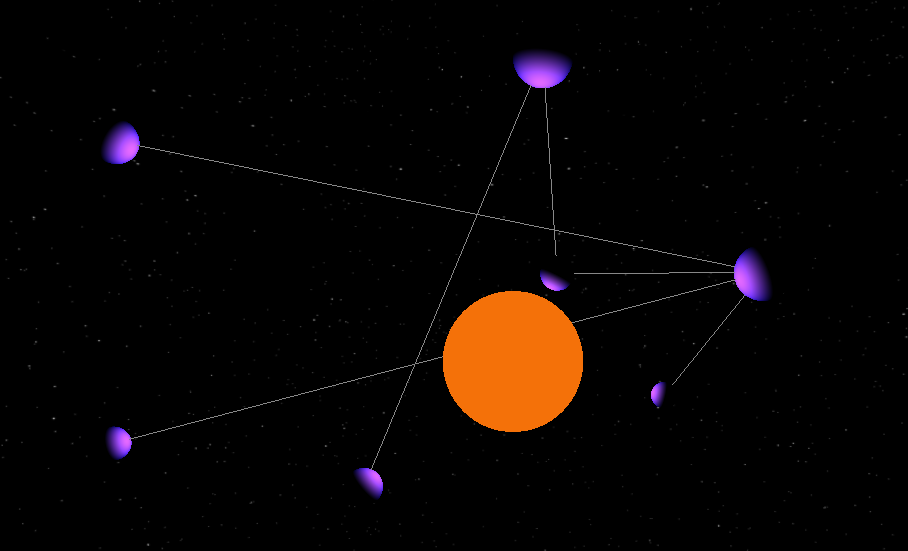
\includegraphics{images/planets.png}
}
\caption{Planetary system}
\label{planets}
\end{figure}
\begin{figure}[H]
\makebox[\textwidth]{
\noindent\resizebox{!}{250pt}{

\includegraphics{images/login_ok.png}
}
\noindent\resizebox{!}{250pt}{

\includegraphics{images/login_error.png}
}
}
\caption{Login form. Valid (left). Invalid (right)}
\label{login_form}
\end{figure}
\begin{figure}[H]
\makebox[\textwidth]{
\begin{minipage}{.5\textwidth}
\begin{figure}[H]
\makebox[\textwidth]{
\noindent\resizebox{!}{250pt}{
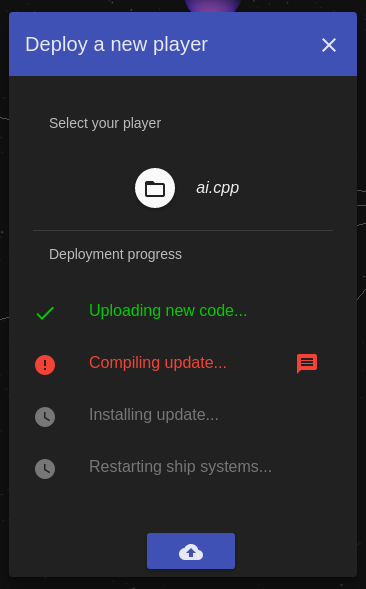
\includegraphics{images/deploy_error.png}
}
}
\caption{Player deployment with a compiling error}
\label{deploy_error}
\end{figure}
\end{minipage}
\begin{minipage}{.5\textwidth}
\begin{figure}[H]
\makebox[\textwidth]{
\noindent\resizebox{!}{100pt}{

\includegraphics{images/game_time.png}
}
}
\caption{Game time}
\label{game_time}
\end{figure}
\end{minipage}
}
\end{figure}
\clearpage
\part{Review}
\chapter{Validation}
\label{methodology}
The \textbf{validation methodology} has changed slightly in order to give priority to \textbf{integration testing}, given that
the platform is made of \textbf{multiple independent components}.

When a change is made to any component while using \textbf{continuous integration}, the change is automatically applied to
the \textbf{latest working prototype}. Therefore, breaking changes can be easily detected. Also, when using  \textbf{continuous
integration} there is always an \textbf{up-to-date} working prototype of the platform that can be shown to anyone.

To set it up, a \href{http://linode.com/}{\textbf{Linode}} running \texttt{Ubuntu} was booted up to execute an instance of
the platform. Then, \href{http://semaphoreci.com/}{\textbf{Semaphore}} was configured to build any change in the
repositories. If a build succeeds, then \textbf{Semaphore} deploys the changes to the \textbf{Linode}, where the changes will
be applied. \autoref{build_process} shows the build process of the \textbf{Space Wars} engine, while
\autoref{deployment_process} shows its deployment process.

Changes are pushed to the \textbf{Linode} using \textbf{bare \texttt{git} repositories} and \textbf{script hooks}. Basically,
when some changes are pushed to the repository, a script is executed that \textbf{builds and restarts the component}.
These scripts are located in the \textbf{repository itself}, so they can be updated easily.
\begin{figure}[H]
\noindent\resizebox{\textwidth}{!}{
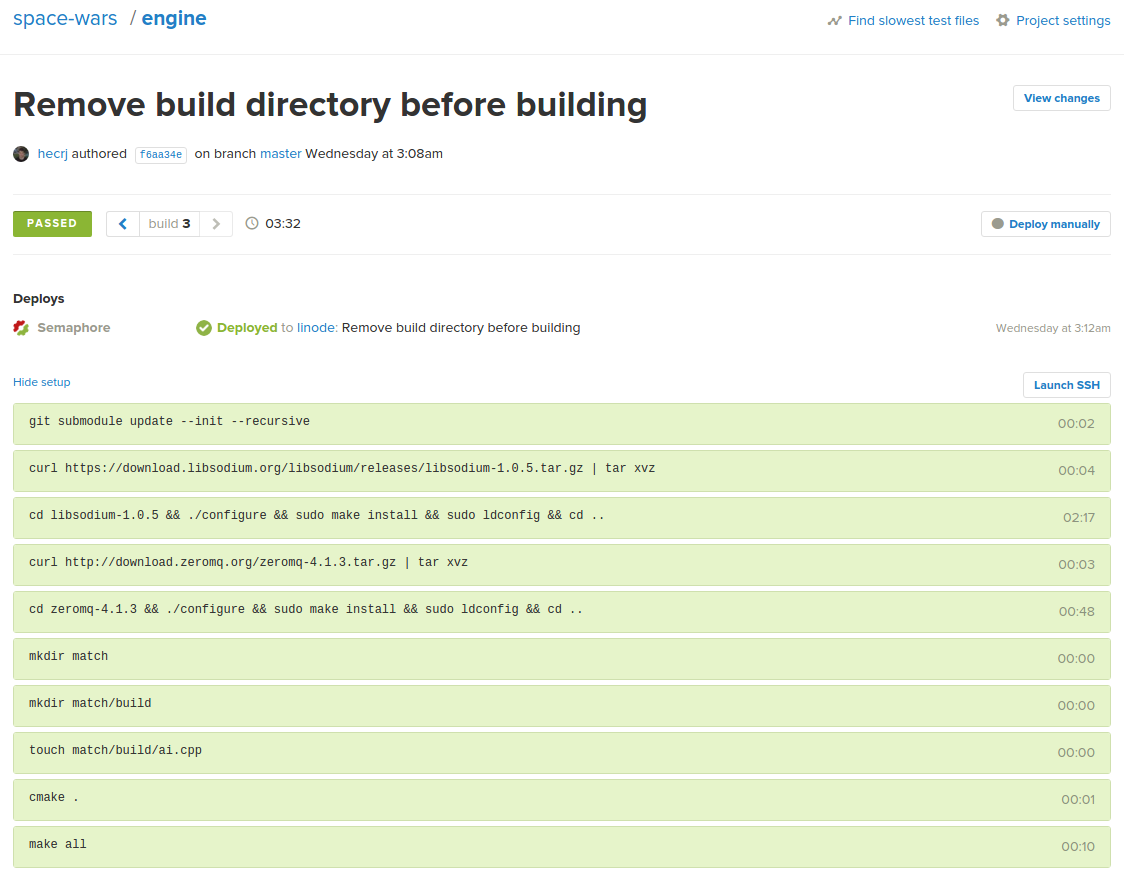
\includegraphics{images/build_process.png}
}
\caption{Semaphore build process}
\label{build_process}
\end{figure}
\begin{figure}[H]
\noindent\resizebox{\textwidth}{!}{
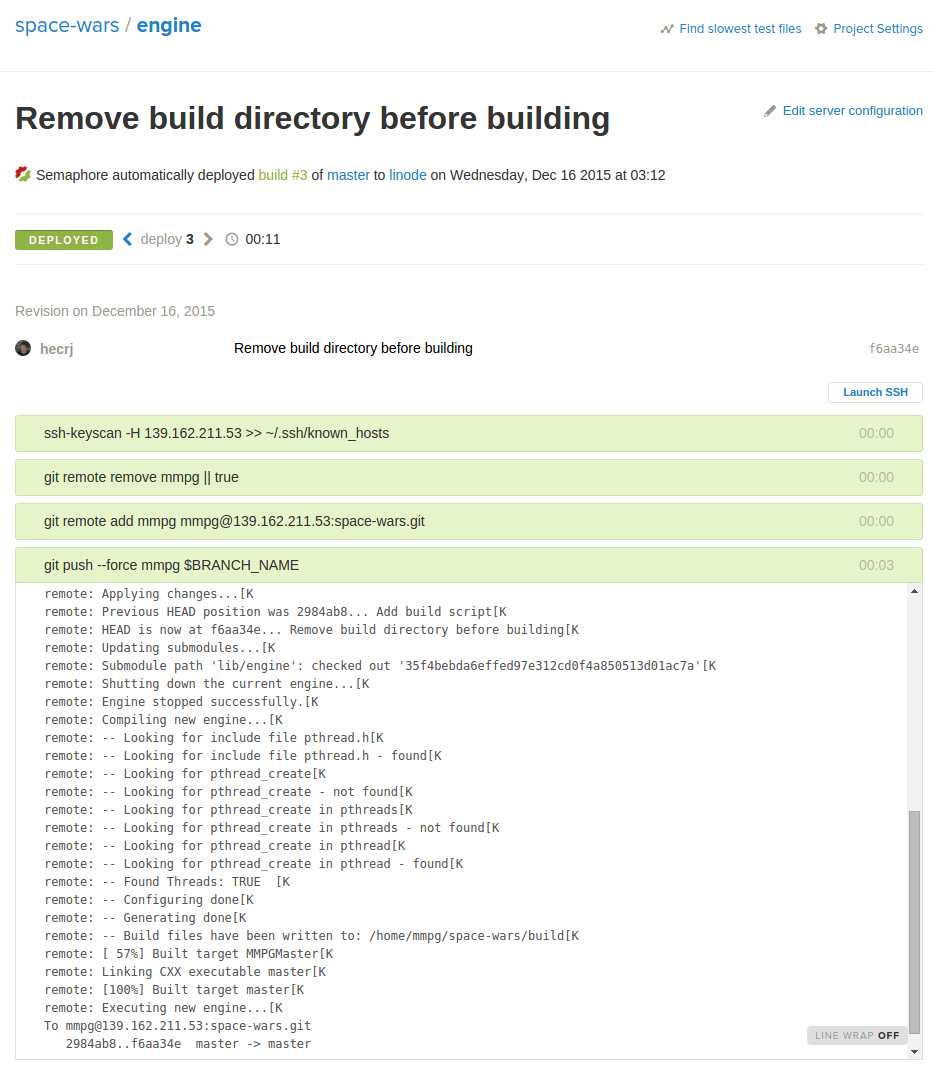
\includegraphics{images/deployment_process.png}
}
\caption{Semaphore deployment process}
\label{deployment_process}
\end{figure}
\clearpage
\chapter{Planning}
\section{Time table}
\label{time_table}
\begin{center}
\begin{tabular}{l | l}
\textbf{Task} & \textbf{Expected duration (h)}\\
\hline
Project management course & 75\\
\hline
Analysis and design & 10\\
\hline
Game engine & -\\
\hspace{1em}
Learning & 5\\
\hspace{1em}
Implementation & 50\\
\hspace{1em}
Testing & 14\\
\hspace{1em}
Integration & 1\\
\hline
Real-time notifier & -\\
\hspace{1em}
Learning & 10\\
\hspace{1em}
Implementation & 25\\
\hspace{1em}
Testing & 10\\
\hspace{1em}
Integration & 5\\
\hline
Notifier subscriber & -\\
\hspace{1em}
Learning & 5\\
\hspace{1em}
Implementation & 20\\
\hspace{1em}
Testing & 3\\
\hspace{1em}
Integration & 2\\
\hline
Control panel & -\\
\hspace{1em}
Learning & 5\\
\hspace{1em}
Implementation & 20\\
\hspace{1em}
Testing & 5\\
\hspace{1em}
Integration & 5\\
\hline
Game example & -\\
\hspace{1em}
Logic & 50\\
\hspace{1em}
Real-time viewer & 50\\
\hline
Testing and polishing & 40\\
\hline
Project memory & 40\\
\hline
Oral presentation & 10\\
\hline
\hline
\textbf{Total} & 460\\
\end{tabular}
\end{center}
The total duration of the project has been \textbf{460 hours}.
\section{Time management}
\begin{figure}[H]
\makebox[\textwidth]{
\noindent\resizebox{300pt}{!}{
\begin{ganttchart}[hgrid, vgrid]{1}{25}
\gantttitle{2015}{20}
\gantttitle{2016}{5}
\\
\gantttitle{September}{5}
\gantttitle{October}{5}
\gantttitle{November}{5}
\gantttitle{December}{5}
\gantttitle{January}{5}
\\
\ganttbar{Project management}{3}{11}
\\
\ganttbar{Analysis and design}{6}{7}
\\
\ganttbar{Engine}{9}{15}
\\
\ganttbar{API}{9}{13}
\\
\ganttbar{Client}{9}{13}
\\
\ganttbar{Space Wars - logic}{16}{19}
\\
\ganttbar{Space Wars - viewer}{16}{20}
\\
\ganttbar{Testing and polishing}{21}{22}
\\
\ganttbar{Project memory}{16}{23}
\\
\ganttbar{Oral presentation}{24}{24}
\ganttlink{elem1}{elem2}
\ganttlink{elem1}{elem3}
\ganttlink{elem1}{elem4}
\ganttlink{elem2}{elem5}
\ganttlink{elem3}{elem6}
\ganttlink{elem4}{elem6}
\ganttlink{elem5}{elem7}
\ganttlink{elem6}{elem7}
\ganttlink{elem8}{elem9}
\end{ganttchart}
}
}
\caption{Final time planning}
\label{gantt_current}
\end{figure}
\section{Dedication}
\autoref{dedication} shows the \textbf{relative amount of contributions per day} to this project.
\begin{figure}[H]
\makebox[\textwidth]{
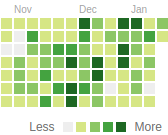
\includegraphics[scale=0.6]{images/dedication.png}
}
\caption{GitHub contributions to the \texttt{MMPG} project \url{https://github.com/hecrj}}
\label{dedication}
\end{figure}
As it can be observed, there is \textbf{at least one contribution per day since November 4}. However, while dedication has
been constant, there are many days where \textbf{contributions were minimal}. Hence, \textbf{dedication and productivity are expected
to increase} during the incoming holidays.
\clearpage
\chapter{Economic cost}
The following resources will be needed to develop the project:
\begin{description}
\item[Hardware]
A computer and \textbf{Jutge.org} servers.
\item[Software]
Ubuntu, Sublime Text, a web-browser, \texttt{CLion}, \LaTeX{}, \texttt{Makefile}, \texttt{git}, \texttt{evince},
  \href{https://github.com/hecrj/hal/raw/master/doc/full/report.pdf}{\texttt{HAL}}, \texttt{C++}, \texttt{Go},
  \texttt{Javascript}, \texttt{Coffeescript}, and \texttt{WebGL}.
\item[Human]
Student, project director, and project management tutor.
\item[Other]
Electricity and internet connection.
\end{description}
\section{Hardware resources}
The project will be developed using a personal desktop computer and a laptop. Also, a monitor,
a keyboard and a mouse are needed to use the desktop computer. There is no other hardware needed.
\begin{table}[H]
\centering
\begin{tabular}{l | S | S | S}
\textbf{Hardware} & \textbf{Cost (\EURtm)} & \textbf{Useful life (years)} & \textbf{Amortized cost (\EURtm)}\\
\hline
Desktop computer & 2600.00 & 4 & 34.13\\
Personal laptop & 1000.00 & 4 & 13.13\\
Monitor Acer XB270HU & 750.00 & 4 & 9.85\\
Mouse Corsair M60 & 60.00 & 4 & 0.79\\
Keyboard Corsair K70 RGB & 170.00 & 4 & 2.23\\
\hline
\hline
\multicolumn{3}{l |}{\textbf{Total}}
 & 60.13
\end{tabular}
\caption{Hardware budget}
\label{Hardware budget}
\end{table}
\section{Software resources}
All the software needed to develop the project can be used for free.
\begin{table}[H]
\centering
\begin{tabular}{l | l}
\textbf{Software} & \textbf{License}\\
\hline
Ubuntu & \url{http://www.ubuntu.com/about/about-ubuntu/our-philosophy}\\
\LaTeX{} & \url{https://latex-project.org/lppl/}\\
\texttt{git} & \url{https://git-scm.com/about/free-and-open-source}\\
\texttt{C++} & \url{https://gcc.gnu.org/onlinedocs/libstdc++/manual/license.html}\\
\texttt{Go} & \url{https://golang.org/project/}\\
Mozilla Firefox & \url{https://www.mozilla.org/en-US/foundation/licensing/}\\
\texttt{Coffeescript} & \url{https://github.com/jashkenas/coffeescript/blob/master/LICENSE}\\
\texttt{WebGL} & \url{https://www.khronos.org/legal/license/}\\
\end{tabular}
\caption{Software licenses}
\label{Software licenses}
\end{table}
Mozilla Firefox includes a \texttt{Javascript} engine and \texttt{evince} is included in Ubuntu.
Also, the \texttt{HAL} programming language is owned by the author of the project. \texttt{Jetbrains} allows students to use
\texttt{CLion} for free\footnote{\url{https://www.jetbrains.com/student/}} and
\texttt{Sublime Text} can be used without registration with no limitations\footnote{\url{http://www.sublimetext.com/2}}.
Therefore, \textbf{there are no software costs}.
\section{Human resources}
\autoref{Tasks per role} shows the tasks assigned to each project role. \autoref{Human resources budget} shows the
expected cost of the human resources according to project roles and their respective tasks.
\begin{table}[H]
\centering
\begin{tabular}{l | l | S}
\textbf{Role} & \textbf{Task} & \textbf{Time (h)}\\
\hline
\multirow{3}{*}{Project manager}
 & Project management course & 75\\
 & Project memory & 40\\
 & Oral presentation & 10\\
\hline
\multirow{1}{*}{Software engineer}
 & Analysis and design & 10\\
\hline
\multirow{6}{*}{Software developer}
 & Game engine & 70\\
 & Real-time notifier & 50\\
 & Notifier subscriber & 30\\
 & Control panel & 35\\
 & Game example & 100\\
 & Testing and polishing & 40\\
\hline
\hline
\multicolumn{2}{l |}{\textbf{Total}}
 & 460.00
\end{tabular}
\caption{Tasks per role}
\label{Tasks per role}
\end{table}
\begin{table}[H]
\centering
\begin{tabular}{l | S | S | S}
\textbf{Role} & \textbf{Payment (\EURtm / h)} & \textbf{Time (h)} & \textbf{Total (\EURtm)}\\
\hline
Project manager & 35.00 & 125 & 4375.00\\
Software engineer & 40.00 & 10 & 400.00\\
Software developer & 30.00 & 325 & 9750.00\\
\hline
\hline
\multicolumn{3}{l |}{\textbf{Total}}
 & 14525.00
\end{tabular}
\caption{Human resources budget}
\label{Human resources budget}
\end{table}
\section{Other resources}
\subsection{Electricity}
Electricity will be needed to power the hardware. \autoref{Electricity budget} shows the power consumption,
the estimated time of usage, and the cost for every piece of hardware that needs an external source of power,
assuming 0.147358 \EURtm / kWh in Spain\footnote{\url{http://comparadorluz.com/faq/precio-kwh-electricidad}}.
\begin{table}[H]
\centering
\begin{tabular}{l | S | S | S}
\textbf{Hardware} & \textbf{Consumption (W)} & \textbf{Time of usage (h)} & \textbf{Cost (\EURtm)}\\
\hline
Desktop computer & 400 & 400 & 23.58\\
Laptop & 100 & 50 & 0.74\\
Monitor Acer XB270HU & 30 & 400 & 1.77\\
\hline
\hline
\multicolumn{3}{l |}{\textbf{Total}}
 & 26.08
\end{tabular}
\caption{Electricity budget}
\label{Electricity budget}
\end{table}
\subsection{Internet connection}
An Internet connection will be necessary to perform all the tasks. The student will use its personal
internet connection most of the time, which costs 38\EURtm/month $\simeq$ 0.05\EURtm/h. It is expected to use the internet connection during the 30\% of the
total project's duration.
Thus, the estimated budget for the internet connection is
460h $\cdot$ 0.05\EURtm/h $\cdot$ 0.3 $=$ \textbf{7.28\EURtm}.
\section{Total}
\autoref{Total budget} shows the total budget needed to develop the project. The 10\% of the total cost
is added to face any unforeseen contingencies.
\begin{table}[H]
\centering
\begin{tabular}{l | S}
\textbf{Resource} & \textbf{Total cost (\EURtm)}\\
\hline
Hardware & 60.13\\
Software & 0.00\\
Human resources & 14525.00\\
Electricity & 26.08\\
Internet & 7.28\\
\hline
\hline
Subtotal & 14618.49\\
Contingency (10\%) & 1461.85\\
\hline
\multicolumn{1}{l |}{\textbf{Total}}
 & 16080.34
\end{tabular}
\caption{Total budget}
\label{Total budget}
\end{table}
\clearpage
\chapter{Sustainability}
This section contains a sustainability report of the project based on the application of the matrix described by
Christian Felber in `The economy of the common good' \cite{sustainability_report}. However, only the \textbf{planning}
stage is considered.
\section{Economic analysis}
The economical analysis is complete and thorough, all costs are assessed and reasonable.
Resources are used efficiently, spending more time in the most important tasks. Moreover, the best technologies
are chosen to produce the best results in the least amount of time possible. A contingency budget has been added
to take care of any unexpected problems. However, the project is not aimed to be profitable, so there will be
no direct economic benefit from it.
\\[0.1cm]
Overall, the project receives a 7 in economical viability because its efficency but lack of profitability.
\section{Social impact analysis}
The project is directed to computer science students and teachers, and game progammers. The project
will be used by students to learn different programming techniques, by teachers to evaluate these students, and
by game programmers to create new content. Moreover, it will be used in the Data Structures and Algorithms subject
at the Barcelona School of Informatics (\textbf{FIB}). The project will make the learning process more fun, it will also
reduce the amount of work for teachers, and it will make game programmers able to create entertaining games easily.
However, the project will not affect the mainstream consumer directly. It will only be relevant inside a specific
community in computer science.
\\[0.1cm]
The project receives a 6 in social impact because it will be positive for a specific community but it will not
have a direct impact on the global population.
\section{Environmental impact analysis}
The project will use 177kWh of electricity, which is approximately 174kg
of CO\textsuperscript{2} \cite{co2}. This is the amount of CO\textsuperscript{2} that a car produces by driving only 7
hours\footnote{\url{http://www.yousustain.com/footprint/howmuchco2?co2=174+kg}}. Also, any source of
information will be accessed digitally over the internet. However, the hardware can not be fully
recycled and it will, eventually, become electronic waste with a high amount of contaminants.
\\[0.1cm]
The project obtains an 8 in environmental impact because its environmental footprint is almost negligible.
\section{Matrix}
\autoref{Sustainability matrix} shows the sustainability matrix and the total score obtained in the planning
stage. The total score obtained is \textbf{21 out of 30}. Therefore, the project is planned to be \textbf{reasonably sustainable}.
\begin{table}[H]
\centering
\begin{tabular}{c | c | c | c | c}
\textbf{Sustainable?} & \textbf{Economic} & \textbf{Social} & \textbf{Environmental} & \textbf{Total}\\
\hline
Planning & 7 & 6 & 8 & \textbf{21}\\
\end{tabular}
\caption{Sustainability matrix}
\label{Sustainability matrix}
\end{table}
\clearpage
\chapter{Legality}
There are no special laws that apply to this project. The entity using the platform
is liable for the information inputted in it, as it is specified in the \textbf{code license}.
\clearpage
\chapter{Conclusion}
...
\clearpage
\bibliographystyle{plain}
\bibliography{references}
\begin{appendices}
...
\clearpage
\end{appendices}
\end{document}
